\documentclass[14pt]{beamer}
\usepackage[T2A]{fontenc}
\usepackage[utf8]{inputenc}
\usepackage[english]{babel}
\usepackage{amssymb,amsfonts,amsmath,mathtext}
\usepackage{cite,enumerate,float,indentfirst}

\usepackage{multicol}
\usepackage{listings}

\renewcommand{\vec}[1]{\ensuremath{\boldsymbol{#1}}}

\graphicspath{{images/}}

\usetheme{Pittsburgh}
\usecolortheme{whale}

\setlength{\columnseprule}{1pt}
\def\columnseprulecolor{\color{blue}}

\setbeamercolor{footline}{fg=blue}
\setbeamertemplate{footline}{
  \leavevmode%
  \hbox{%
  \begin{beamercolorbox}[wd=.333333\paperwidth,ht=2.25ex,dp=1ex,center]{}%
    Boris Kudryashov, ITMO University
  \end{beamercolorbox}%
  \begin{beamercolorbox}[wd=.333333\paperwidth,ht=2.25ex,dp=1ex,center]{}%
    St. Petersburg, 2016
  \end{beamercolorbox}%
  \begin{beamercolorbox}[wd=.333333\paperwidth,ht=2.25ex,dp=1ex,right]{}%
  Page \insertframenumber{} of \inserttotalframenumber \hspace*{2ex}
  \end{beamercolorbox}}%
  \vskip0pt%
}

\newcommand{\itemi}{\item[\checkmark]}

\title{\small{Information Theory. 5th Chapter Slides}}
\author{\huge{
Boris Kudryashov \\
\vspace{30pt}
ITMO University
}}

% \hyperlink{refthis}{here}
% \hypertarget{refthis}{}


\begin{document}

\maketitle

  

\begin{frame}
\frametitle{Agenda}
\begin{enumerate}
% \footnotesize {
\small{
    \item{Noiseless coding problem statement}
    \item{Channel models}
    \item{Mutual information. Average mutual information}
    \item{Conditional average mutual information. Information rework theorem}
    \item{Convexity of average mutual information}
    \item{Information capacity and throughput}
    \item{Fano inequality}
    \item{Reverse coding theorem}
    \item{Information capacity of memoryless channels}
    \item{Symmetrical channels}
    \item{Forward Coding Theorem}
    \item{Typical Sequence pairs}
}

\end{enumerate}
\end{frame}


\begin{frame}
\frametitle{Noiseless coding problem statement}
\begin{itemize}

% \footnotesize {
% \small{
    \item $X=\{0, 1\}. Y = X$
    \item Discrete channel with noise.
    \item Develop a code to eliminate errors.
    
    
    \pause
    \begin{table}[htbp]
    \begin{center}
    \caption{Example 1}
    \begin{tabular}
        {|c|c|c|} \hline %
        Message & Codeword & Decisive area \\ \hline %
        0& 000&   {\{}000, 001, 010, 100{\}} \\ \hline %
        1& 111&   {\{}011, 101, 110, 111{\}} \\ \hline %
    \end{tabular}
    \end{center}
    \end{table}
    

% }
\end{itemize}
\end{frame}



\begin{frame}
\frametitle{Noiseless coding problem statement}

% \footnotesize {
% \small{

   
    \begin{table}[htbp]
    \begin{center}
    \caption{Example 2}
    \begin{tabular}
        {|c|c|c|} \hline %
        Message & Codeword & Decisive area \\ \hline %
        00& 00000& \{00000,00001,00010,00100,  \\
          &      &   01000,10000,11000,10001\} \\  \hline %
        01& 10110& \{10110,10111,10100,10010, \\
          &      &   11110,00110,01110,00111\} \\  \hline %
        10& 01011& \{01011,01010,01001,01111,  \\
          &      &   00011,11011,10011,11010\} \\  \hline %
        11& 11101& \{11101,11100,11111,11001,  \\
          &      &   10101,01101,00101,01100\} \\ \hline %
    \end{tabular}
    \end{center}
    \end{table}

\end{frame}



\begin{frame}
\frametitle{Noiseless coding problem statement}
\begin{itemize}
% \footnotesize {
\small{

    \item
        \begin{figure}[ht]
        \begin{minipage}{1.0\linewidth}
        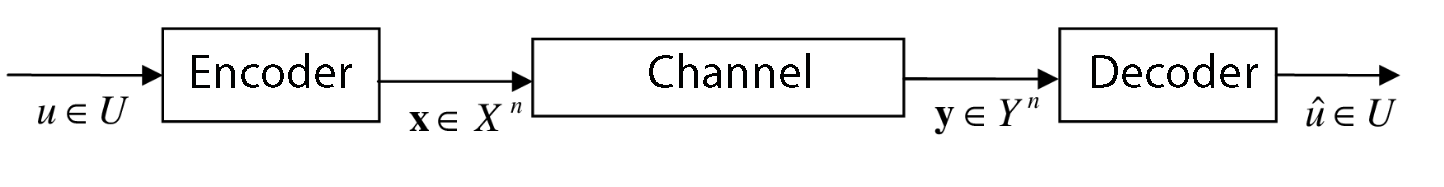
\includegraphics[width=1.0\textwidth]{fig5_1.png}
        %\centerline{\includegraphics[width=3.16in,height=4.02in]
        \caption{Communication system Scheme}
        \label{fig5_1}
        \end{minipage}
        \end{figure}    

    \pause 
    \item
        \textit{Code of channel} over $X$ is arbitrary set of sequences $A = \{{\vec x}_m \}$, $m = 1,...,M$, $A \in X^n$. 
    \item    
        These sequences are \textit{codewords}.
    \item    
        Their length $n$ is \textit{code length}. 
    \item   
        Number of sequences $M$ is \textit{code cardinality}.
        $R$, defined as:
        \begin{equation}
            R = \frac{\log M}{n}
        \end{equation}
        is called \textit{code rate} (bits per symbol).
    \item 
        Event when $\hat {u} \ne u$ is \textit{decoding error}.
    \item 
        And it's probability is \textit{error probability}
}
\end{itemize}
\end{frame}


% --------------------Channel models----------

\begin{frame}
\frametitle{Channel models}
\begin{itemize}
% \footnotesize {
% \small{
\item
    \textit{Channel model} is defined, if $\forall  n$ and $\forall  {\vec x} \in X^n$, ${\vec y} \in Y^n$ conditional probability $p({\vec y}\vert {\vec x})$ is defined.

\pause \item
    Reminder: ${\vec x}_i^n = (x_i ,...,x_n )$. 
    Channel is called \textit{stationary}, if $\forall  j, n $ and $ \forall {\vec x}_{j + 1}^{j + n} \in X^n$, ${\vec y}_{j + 1}^{j + n} \in Y^n$ conditional probabilities $p({\vec y}_{j + 1}^{j + n} \vert {\vec x}_{j + 1}^{j + n} )$ are defined by sequence characters and do not depend from index $j$.

\end{itemize}
\end{frame}


\begin{frame}
\frametitle{Channel models}
\begin{itemize}

\item
Channel is called \textit{memoryless}, if $\forall j,n $ and $\forall {\vec x}_{j + 1}^{j + n} \in X^n$, ${\vec y}_{j + 1}^{j
+ n} \in Y^n$
\[
p({\vec y}_{j + 1}^{j + n} \vert {\vec x}_{j + 1}^{j + n} ) =
\prod\limits_{i = j + 1}^{j + n} {p(y_i \vert x_i )} .
\]


\pause \item
Stationary channel without memory is called discrete stationary channel.

\end{itemize}
\end{frame}


\begin{frame}
\frametitle{Channel models}
\begin{itemize}
% \footnotesize {
% \small{
To describe a Discrete Stationary Channel it's enough to define conditional probabilities $\{p(y\vert x),x \in X,y \in Y\}$. Let $X = \{0,...,K - 1\}$, $Y = \{0,...,L - 1\}$. Let $p_{ij} = p(y = j\vert x = i\}$, $i \in X$, $j \in Y$. 
Describe transition probabilities of channel $p_{ij} $ in a \textit{transition probability matrix}:
\[
\left[
  \begin{array}{cccc}
    p_{00} & p_{01} & \cdots & p_{0,L - 1} \\
    p_{10} & p_{11} & \cdots & p_{1,L - 1} \\
    \vdots & \vdots & \ddots & \vdots \\
    p_{K - 1,0} & p_{K - 1,1} & \cdots & p_{K - 1,L - 1} \\
  \end{array}
\right].
\]

\end{itemize}
\end{frame}


\begin{frame}
\frametitle{Channel models}
\begin{itemize}
% \footnotesize {
% \small{

\begin{figure}[ht]
\begin{minipage}{1.0\linewidth}
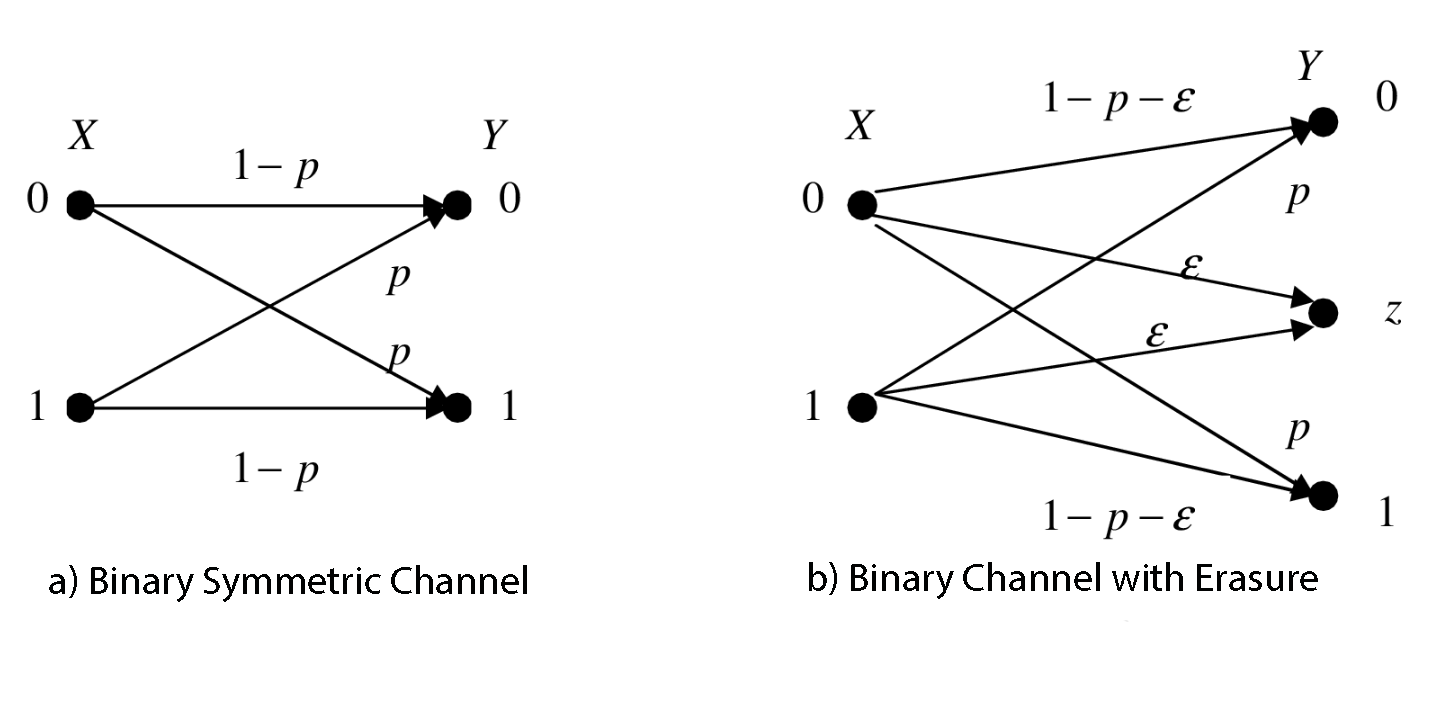
\includegraphics[width=1.0\textwidth]{fig5_2.png}
%\centerline{\includegraphics[width=3.16in,height=4.02in]
\caption{Discrete stationary channels examples} \label{fig5_2}
\end{minipage}
\end{figure}

\end{itemize}
\end{frame}

\begin{frame}
\frametitle{Channel models}
\begin{itemize}
% \footnotesize {
% \small{
    \item Binary Symmetric Channel (BSC).
        $X = Y = \{0,1\}$,
        $p_{10} = p_{01} = p$, $p_{00} = p_{11} = 1 - p$. 
        Transition probability matrix: 
        \[
        P = \left[ {{\begin{array}{*{20}c}
         {1 - p} \hfill & p \hfill \\
         p \hfill & {1 - p} \hfill \\
        \end{array} }} \right].
        \]

    \pause \item
    Binary Symmetric Channel with Erasure (BSCE). 
    \[
    P = \left[ {{\begin{array}{*{20}c}
     {1 - p - \varepsilon } \hfill \\
     p \hfill \\
    \end{array} }\mbox{ }{\begin{array}{*{20}c}
     \varepsilon \hfill \\
     \varepsilon \hfill \\
    \end{array} }\mbox{ }{\begin{array}{*{20}c}
     p \hfill \\
     {1 - p - \varepsilon } \hfill \\
    \end{array} }} \right].
    \]
    $X = {0,1}, Y = {0, 1, z}$, where $z$ is a special erasure symbol.    
    
\end{itemize}
\end{frame}

% ------------------Mutual information---------------

\begin{frame}
\frametitle{Mutual information}
\begin{itemize}
% \footnotesize {
% \small{

    \item
    For a given $XY = \{(x,y),p(x,y)\}$ of ensembles $X$ and $Y$ calculate the information about $x \in X$ by $y \in Y$.
    
    \pause \item
    Mutual information:
    \begin{equation}
    \label{eq5_2} I(x;y) = I(x) - I(x\vert y).
    \end{equation}
    
    
    
\end{itemize}
\end{frame}


\begin{frame}
\frametitle{Mutual information}
\begin{itemize}
% \footnotesize {
% \small{    
    \item
    \textit{Average mutual information} of $X$ and $Y$ is
    \[
    I(X;Y) = {\rm {\bf M}}\left[ {I(x;y)} \right].
    \]
    
    \pause \item
    Dependence between average mutual information and joint probability distribution:
    \begin{equation}
    \label{eq5_3} I(X;Y) = \sum\limits_{x \in X} {\sum\limits_{y \in
    Y} {p(x,y)\log \frac{p(y\vert x)}{p(y)}} } .
    \end{equation}
    
\end{itemize}
\end{frame}


\begin{frame}
\frametitle{Mutual information}
Properties of mutual information:

\begin{enumerate}
% \footnotesize {
% \small{

    \item[1]
    \begin{prop} \label{p5_1}
    Symmetricity: $I(x;y) = I(y;x)$.
    \end{prop}
    
    \pause \item[2] 
    \begin{prop} \label{p5_2}
    If $x$ and $y$ are independent, $I(x,y) = 0$.
    \end{prop}
    
    \pause \item[3] 
    \begin{prop} \label{p5_3}
    Symmetricity $I(X;Y) = I(Y;X)$\textbf{.}
    \end{prop}
    
    \pause \item[4] 
    \begin{prop} \label{p5_4}
    Nonnegativity: $I(X;Y) \ge 0$.
    \end{prop}
    
    \pause \item[5] 
    \begin{prop} \label{p5_5}
    Identity $I(X;Y) = 0$ holds iff  ensembles $X$ and $Y$ are independent.
    \end{prop}
    
    
\end{enumerate}
\end{frame}


\begin{frame}
\frametitle{Mutual information}
Properties of mutual information:

\begin{enumerate}
% \footnotesize {
    
    \item[6] 
    \begin{prop} \label{p5_6}
    $I(X;Y) = H(X) - H(X\vert Y) = H(Y) - H(Y\vert X) =H(X) + H(Y) - H(XY).$
    \end{prop}
    
    
    \pause \item[7] 
    \begin{prop} \label{p5_7}
    $I(X;Y) \le \min \left\{ {H(X),H(Y)} \right\}.$
    \end{prop}
    
    \pause \item[8] 
    \begin{prop} \label{p5_8}
    $I(X;Y) \le \min \left\{ {\log \vert X\vert ,\log \vert Y\vert } \right\}.$
    \end{prop}
    
    \pause \item[9] 
    \begin{prop}  \label{p5_9}
    Mutual information $I(X;Y)$ is a convex $ \cap $ function of probability distribution $p(x)$.
    \end{prop}
    
    \pause \item[10] 
    \begin{prop}  \label{p5_10}
    Mutual information $I(X;Y)$ is a convex $ \cup $ function of conditional probabilities $p(y\vert x)$.
    \end{prop}    
    

\end{enumerate}
\end{frame}

% ----------------Conditional average mutual information------

\begin{frame}
\frametitle{Conditional average mutual information.}
\begin{itemize}
% \footnotesize {
% \small{
    \item 
    Consider $XYZ = \{(x,y,z),p(x,y,z)\}.$ 
    Fix $z \in Z$ and consider conditional probability distribution:
    $p(x,y\vert z) = \frac{p(x,y,z)}{p(z)}.$

    \item   
    Average mutual information between $X$ and $Y$:
    $ I(X;Y\vert z) = \sum\limits_{x \in X} {\sum\limits_{y \in Y} {p(x,y\vert z)\log \frac{p(y\vert x,z)}{p(y\vert z)}} }.$

\end{itemize}
\end{frame}


\begin{frame}
\frametitle{Conditional average mutual information.}
\begin{itemize}
% \footnotesize {
% \small{
    \item
    Conditional average mutual information between $X$ and $Y$:
    
    $I(X;Y\vert Z) = {\rm {\bf M}}\left[ {I(X;Y\vert z} \right] = \sum\limits_{x \in X} {\sum\limits_{y \in Y} {\sum\limits_{z \in Z} {p(x,y,z)} \log \frac{p(y\vert x,z)}{p(y\vert z)}} }$
    
    \item
    Additional properties:
    $I(X;Y\vert Z) = H(Y\vert Z) - H(Y\vert XZ).$
    $I(X;YZ) &=& I(X;Y) + I(X;Z\vert Y)$
    $I(X;YZ) &=& I(X;Z) + I(X;Y\vert Z)$
\end{itemize}
\end{frame}

\begin{frame}
\frametitle{Conditional average mutual information.}
\begin{itemize}
% \footnotesize {
% \small{
    A special case of information processing system, which has 3 probability ensembles:
    \begin{figure}[ht]
    \begin{minipage}{1.0\linewidth}
    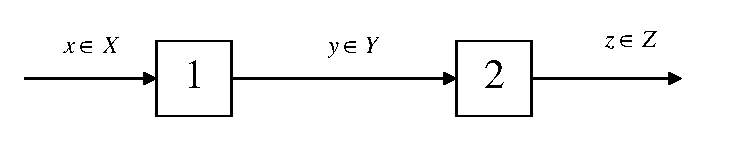
\includegraphics[width=1.0\textwidth]{fig5_3.eps}
    \caption{Information processing system} \label{fig5_3}
    \end{minipage}
    \end{figure}
\end{itemize}
\end{frame}

\begin{frame}
\frametitle{Conditional average mutual information.}
\begin{itemize}
% \footnotesize {
% \small{

    \begin{theorem}
    \label{th_inf_trans} Let $X$, $Y$, $Z$ be probability ensembles,
    which are formed by the information processing system at the previous slide. Then holds:
    \begin{eqnarray}
    \label{eq5_8} I(X;Y) &\ge& I(X;Z),\\
     \label{eq5_9} I(Y;Z) &\ge& I(X;Z).
    \end{eqnarray}
    \end{theorem}

\end{itemize}
\end{frame}


\begin{frame}
\frametitle{Conditional average mutual information.}
% \footnotesize {
% \small{

    \textbf{proof.} Use properties of conditional average mutual information:
    \begin{eqnarray}
    \label{eq5_10} I(X;YZ) &=& I(X;Y) + I(X;Z\vert Y), \\
    \label{eq5_11} I(X;YZ) &=& I(X;Z) + I(X;Y\vert Z).
    \end{eqnarray}
    $X$ and $Z$ are independent. If $Y$ is known, \\
    $I(X;Z\vert Y) = 0$. 
    By equating the right sides of (\ref{eq5_10}) and
    (\ref{eq5_11}), we get
    \[
    I(X;Y) = I(X;Z) + I(X;Y\vert Z).
    \]
    Since the second term is non-negative, we obtain the inequality
    (\ref{eq5_8}). Similarly we can prove (\ref{eq5_9}). 

\end{frame}



% ----------------Convexity of average mutual information---------

\begin{frame}
\frametitle{Convexity of average mutual information}
\begin{itemize}
% \footnotesize {
 \small{

    \item Let ${\vec p} = (p_0 ,...,p_{K - 1} )$ be probabilities of input symbols $X = \{0,...,K - 1\}$. Let use $I({\vec p})$ instead of $I(X;Y)$ to emphasize that we are interested in the dependence between mutual information and input symbols distribution.
    
    \item Consider $Z = \{1,2\}$ such that $p_z(1) = \alpha$, $p_z(2)=1-\alpha$
    
    \item Consider $XYZ$, where tuples $(x,y,z)$ are created as follows: \\
    (1) $z$ is chosen according to $p(z)$. \\
    (2) if $z = 1, p_1$ is used to choose $x$, otherwise, $p_2$ is used.\\
    (3) After that, according to $p(y|x)$, $y$ element is generated.\\
}
\end{itemize}
\end{frame}



\begin{frame}
\frametitle{Convexity of average mutual information}
\begin{itemize}
% \footnotesize {

    \item From the convexity definition: $\forall p_1, p_2, \alpha \in [0,1]$ holds
    \begin{equation} \label{eq5_12}
        I\left( {\alpha {\vec p}_1 + (1 - \alpha ) {\rm {\bf p}}_2 } \right) 
        \ge \alpha I({\vec p}_1 ) + (1 - \alpha ) I ({\vec p}_2 ).
    \end{equation}
    
    \item According to previous definitions:
    \[
    \begin{array}{lll}
        I(X;Y\vert z = 1) &=& I({\vec p}_1 );\\
        I(X;Y\vert z = 2) &=& I({\vec p}_2 );\\
        I(X;Y\vert Z) &=& \alpha I({\vec p}_1 ) + (1 - \alpha )%
        I({\vec p}_2 );\\
        I(X;Y) &=& I\left( {\alpha {\vec p}_1 + (1 - \alpha ){\vec p}_2 } \right).
    \end{array}
    \]
    
    \item Inequation (\ref{eq5_12}) is reduced to:
    \begin{equation}
        \label{eq5_13} I(X;Y) \ge I(X;Y\vert Z).
    \end{equation}
    

\end{itemize}
\end{frame}


\begin{frame}
\frametitle{Convexity of average mutual information}
\begin{itemize}
% \footnotesize {


    \item consider mutual information $I(Y;XZ)$:
    \begin{eqnarray}
        \label{eq5_14} I(Y;XZ) &=& I(Y;X) + I(Y;Z\vert X); \\
        \label{eq5_15} I(Y;XZ) &=& I(Y;Z) + I(Y;X\vert Z).
    \end{eqnarray}
    
    \item As long as $Z$ and $Y$ are independent, $I(Y;Z\vert X) = 0$
    
    \item By equating the right sides, we get (\ref{eq5_13}). \QED


\end{itemize}
\end{frame}


\begin{frame}
\frametitle{Convexity of average mutual information}
\begin{itemize}
% \footnotesize {
\small{

    \item Consider mutual information as function of conditional distribution $p(y|x)$.
    
    \item $\forall P_1, P_2, \alpha \in [0,1]$ holds:
    \begin{equation}
        \label{eq5_16} I\left( {\alpha P_1 + (1 - \alpha )P_2 } \right)
        \le \alpha I(P_1 ) + (1 - \alpha )I(P_2 ).
    \end{equation}

    \item Consider $Z=\{1,2\}$. Consider $XYZ$, where tuples $(x,y,z)$ are created as follows: \\
    (1) $x \in X$ is chosen according to $p(x)$. \\
    (2) $z$ is chosen according to $p(z)$. \\
    (3) Transition probability matrix P is chosen: $P = P_1 (if z = 1 ) or P = P_2 (if z = 2)$
    (4) After that, according to $x$ and $P$, $y$ element is generated.\\
    
}    
\end{itemize}
\end{frame}



\begin{frame}
\frametitle{Convexity of average mutual information}
\begin{itemize}
% \footnotesize {
% \small{

    \item According to previous definitions:
    \[
    \begin{array}{lll}
    I(X;Y\vert z = 1) &=& I(P_1 );\\
    I(X;Y\vert z = 2)  &=& I(P_2 );\\
    I(X;Y\vert Z) &=& \alpha I(P_1 ) + (1 - \alpha )I(P_2 );\\
    I(X;Y) &=& I\left( {\alpha P_1 + (1 - \alpha )P_2 } \right).
    \end{array}
    \]
    
    \item (\ref{eq5_16}) is now reduced to 
    \begin{equation}
        \label{eq5_17} I(X;Y) \le I(X;Y\vert Z).
    \end{equation}
    
\end{itemize}
\end{frame}



\begin{frame}
\frametitle{Convexity of average mutual information}
\begin{itemize}
% \footnotesize {
% \small{
    
    \item Rewrite mutial information in two ways:
    \begin{eqnarray}
        \label{eq5_18} I(X;YZ) &=& I(X;Y) + I(X;Z\vert Y);\\
        \label{eq5_19} I(X;YZ) &=& I(X;Z) + I(X;Y\vert Z).
    \end{eqnarray}

    \item By equating the right sides (\ref{eq5_18}) and (\ref{eq5_19}), we get (\ref{eq5_17}) and (\ref{eq5_16}). Thus, we prooved convexity $ \cup $ of mutual information as a function of conditional distributions. \QED
    
    

\end{itemize}
\end{frame}


% -----------------Information capacity and throughput--------------------

\begin{frame}
\frametitle{Information capacity and throughput}
\begin{itemize}
% \footnotesize {
% \small{
    
    \item When using codewords of length $n$, average amount of information, received by decoder will be $I(X^n;Y^n)$ bit. This corresponds to information rate: 
    \[
    \frac{1}{n}I(X^n;Y^n) \mbox{bit/channel symbol}.
    \]

    \item $C_0$ is called the Information Capacity of channel.
    \begin{equation}
        \label{eq5_20}
        C_0 = \mathop {\sup }\limits_n \mathop {\max }%
        \limits_{\left\{ {p(\vec x)} \right\}} \frac{1}{n}I(X^n;Y^n)
    \end{equation}
        
\end{itemize}
\end{frame}

% -------------------------Fano inequality--------------------------

\begin{frame}
\frametitle{Fano inequality}
\begin{itemize}
% \footnotesize {
% \small{

\begin{figure}[ht]
\begin{center}
\begin{minipage}{0.6\linewidth}
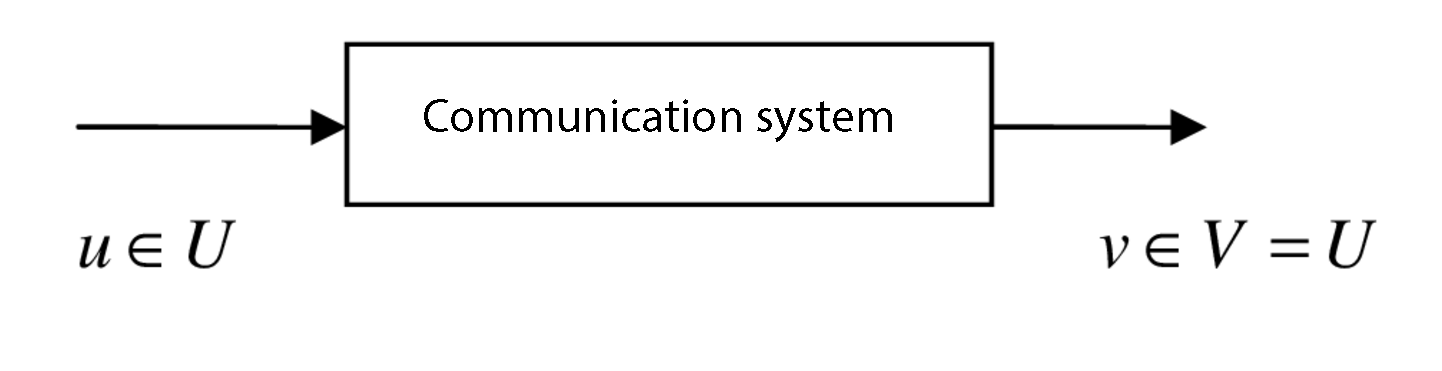
\includegraphics[width=1.0\textwidth]{fig5_4.png}
\caption{Information transfer system} \label{fig5_4}
\end{minipage}
\end{center}
\end{figure}

    \item Messages are elements of $U = \{u\} = \{0,...,M - 1\}$.
    \item Receiver gets estimates of messages.
    \item Estimates are denoted $V = \{v\}$. 
    \item $U$ and $V$ are bijective. 
    \item If $u \ne v$ there is a decoding error.

\end{itemize}
\end{frame}



\begin{frame}
\frametitle{Fano inequality}
\begin{itemize}
% \footnotesize {
% \small{
    \item $UV = \left\{ {(u,v),p(u,v)} \right\}$ and $p(u,v)$ are known.
    
    \item Error probability $P_e $ is
    \begin{equation}
        \label{eq5_21} P_e = \sum\limits_u {\sum\limits_{v \ne u} {p(u,v)}}.
    \end{equation}

    \item Probability of correct decoding: 
    \begin{equation}
        \label{eq5_22} P_c = 1 - P_e = \sum\limits_u {\sum\limits_{v = u} {p(u,v)}}.
    \end{equation}
    
\end{itemize}
\end{frame}


\begin{frame}
\frametitle{Fano inequality}
\begin{itemize}
% \footnotesize {
% \small{

\begin{theorem}(Fano inequality)
    \begin{equation}
    \label{eq5_23} H(U\vert V) \le \eta(P_e ) + P_e \log (M - 1),
    \end{equation}
    where $\eta(\cdot)$ denotes entropy of binary ensemble.
    \label{th_fano}
\end{theorem}

\end{itemize}
\end{frame}


\begin{frame}
\frametitle{Fano inequality}
\begin{itemize}
% \footnotesize {
% \small{
Consider right side of Fano Inequality.
\begin{equation}
\label{eq5_24} \gamma (P_e ) = \eta(P_e ) + P_e \log (M - 1)
\end{equation}

\begin{center}
\begin{figure}[ht]
\begin{minipage}{1.0\linewidth}
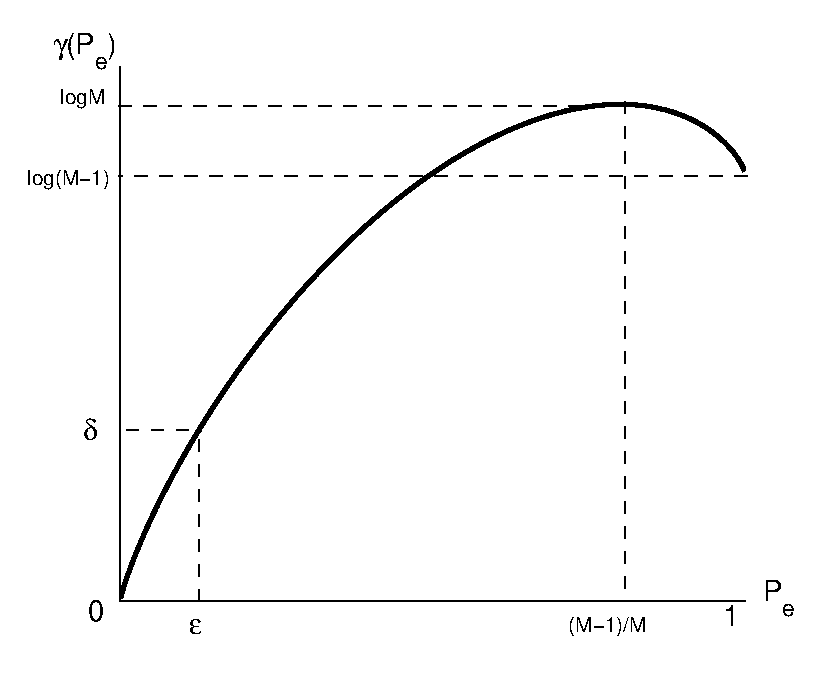
\includegraphics[width=0.75\textwidth]{fano.eps}
\caption{Right side of Fano Inequality} \label{fano}
\end{minipage}
\end{figure}
\end{center}


\end{itemize}
\end{frame}





\begin{frame}
\frametitle{Fano inequality}

Proof of Fano Inequality \ref{th_fano}. 
\begin{itemize}

% \small{
    
    \item
    Use (\ref{eq5_21}) and (\ref{eq5_22}), rewrite terms of (\ref{eq5_23}):
    
\footnotesize {    
    \begin{equation}
    \label{eq5_25} H(U\vert V) = - \sum\limits_u {\sum\limits_{v \ne
    u} {p(u,v)\log p(u\vert v)} } - \sum\limits_u {\sum\limits_{v = u}
    {p(u,v)\log p(u\vert v)} } ,
    \end{equation}
    

    \begin{equation}
    \label{eq5_26} \eta(P_e ) = - \sum\limits_u {\sum\limits_{v \ne u}
    {p(u,v)\log P_e - } } \sum\limits_u {\sum\limits_{v \ne u}
    {p(u,v)\log P_c } } ,
    \end{equation}


    \begin{equation}
    \label{eq5_27} P_e \log (M - 1) = \sum\limits_u {\sum\limits_{v
    \ne u} {p(u,v)\log (M - 1)} } .
    \end{equation}
}
\end{itemize}
\end{frame}

\begin{frame}
\frametitle{Fano inequality}
\begin{itemize}
% \footnotesize {
% \small{

    \item Consider $\Delta$. For (\ref{eq5_23}), we need to prove $\Delta \le 0$.
    \[
    \Delta = H(U\vert V) - \eta(P_e ) - P_e \log (M - 1).
    \]
    
    \item Subtract from (\ref{eq5_25}) corresponding parts of (\ref{eq5_26}) and (\ref{eq5_27}).
    \footnotesize {
    \[
    \Delta = \sum\limits_u {\sum\limits_{v \ne u} {p(u,v)\log \frac{P_e}{p(u\vert v)(M - 1)} + } } \sum\limits_u {\sum\limits_{v = u} {p(u,v)\log \frac{P_c }{p(u\vert v)}} } .
    \]
    }
    \normalsize
    
    \item Use $ \log x \le (x - 1)\log e$
    \footnotesize {
    \[
    \Delta \le (\log e) \left[%
    \sum_u \sum_{v \ne u} p(u,v)\frac{P_e }{p(u\vert v)(M - 1)} - %
    \sum_u \sum_{v \ne u} {p(u,v)} + \right.
    \]
    \[
    \left. %
    +\sum_u \sum_{v = u} p(u,v)\frac{P_c }{p(u\vert v)} - %
    \sum_u \sum_{v = u} p(u,v) \right].
    \]
    }

\end{itemize}
\end{frame}



\begin{frame}
\frametitle{Fano inequality}
\begin{itemize}
% \footnotesize {
% \small{   
    
    \item Use $p(u,v) = p(v)p(u\vert v)$ and (\ref{eq5_21}) и (\ref{eq5_22}).
    \footnotesize {
    \begin{equation}
    \label{eq5_28} \Delta \le \log e\times \left[ {\frac{P_e }{M -
    1}\sum\limits_u {\sum\limits_{v \ne u} {p(v) - P_e + } } P_c
    \sum\limits_u {\sum\limits_{v = u} {p(v) - P_c } } } \right].
    \end{equation}  
    
    
    \item Note, that 
    \begin{equation}
    \label{eq5_29} \sum\limits_u {\sum\limits_{v \ne u} {p(v) = (M - 1)\sum\limits_v {p(v) = (M - 1)} } } .
    \end{equation}

    \item Moreover 
    \begin{equation}
    \label{eq5_30} \sum\limits_u {\sum\limits_{v = u} {p(v) =
    \sum\limits_u {p(u) = 1} } } .
    \end{equation}

    \item Substitute (\ref{eq5_29}) and (\ref{eq5_30}) in (\ref{eq5_28}) and get $\Delta \le 0$. \QED

}
\end{itemize}
\end{frame}



\begin{frame}
\frametitle{Fano inequality}
\begin{itemize}
% \footnotesize {
% \small{

    \begin{figure}[ht]
    \begin{center}
    \begin{minipage}{0.8\linewidth}
    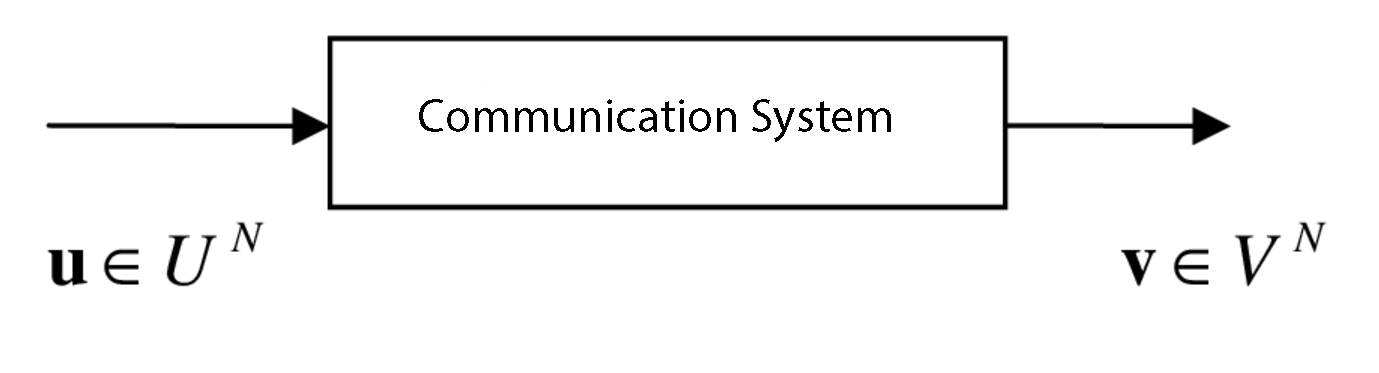
\includegraphics[width=0.8\textwidth]{fig5_6.png}
    \caption{Система передачи информации} \label{fig5_6}
    \end{minipage}
    \end{center}
    \end{figure}
    
    \item Let input be a sequence of messages ${\vec u} = (u_1 ,...,u_N)$
    \item Let output be a sequence of decisions ${\vec v} = (v_1,...,v_N )$
    \item $u_i ,v_i \in U = V = \{0,...,M - 1\}$, $i = 1,...,N$
    \item Let error probability in $i$-th message be $P_{ei} = P(u_i \ne v_i )$

\end{itemize}
\end{frame}




\begin{frame}
\frametitle{Fano inequality}
\begin{itemize}
% \footnotesize {
% \small{

    \item Let Average error probability of sequence of length $N$ be
    \[
    \bar {P}_e = \frac{1}{N}\sum\limits_{i = 1}^N {P_{ei} } .
    \]


    \begin{theorem} \label{th_fano_seq}For sequences $({\vec u},\vec v) \in U^NV^N$, which consist of elements of $M$, holds
    \begin{equation}
    \label{eq5_31} \frac{1}{N}H(U^N\vert V^N) \le \eta(\bar {P}_e ) +
    \bar {P}_e \log (M - 1)
    \end{equation}
    \end{theorem}

\end{itemize}
\end{frame}




\begin{frame}
\frametitle{Fano inequality}
\begin{itemize}
% \footnotesize {
% \small{

    
    \item Use properties of Conditional Entropy
    \footnotesize {
    \[
    H(U^N\vert V^N) = \sum\limits_{i = 1}^N {H(U_i \vert U_1 ...U_{i - 1} V^N)
    \le } \sum\limits_{i = 1}^N {H(U_i \vert V_i )} .
    \]
    }

    \item \normalsize Divide both sides on $N$ and use Fano Inequality
    \footnotesize {
    \[
    \frac{1}{N}H(U^N\vert V^N) \le \frac{1}{N}\sum\limits_{i = 1}^N
    {\eta(P_{ei} ) + } \frac{1}{N}\sum\limits_{i = 1}^N {P_{ei} \log (M
    - 1)} .
    \]
    }
    
    \item \normalsize As long as entropy is convex $ \cap $ function, we get (\ref{eq5_31}) from the last inequality. \QED



\end{itemize}
\end{frame}




\begin{frame}
\frametitle{Reverse coding theorem}
\begin{itemize}
% \footnotesize {
% \small{

    \begin{theorem} {Reverse coding theorem.} For Discrete Memoryless Channel with information capacity $C_0 $, $\forall$ $\delta > 0$ $\exists$ $\varepsilon > 0$, such that $\forall$ code with code rate $R > C_0 + \delta $ average error probability satisfies the inequality:
    \[
    \bar {P}_e \ge \varepsilon .
    \]
    \end{theorem}


\end{itemize}
\end{frame}


\begin{frame}
\frametitle{Reverse coding theorem}
 Proof of Reverse Coding Theorem
\begin{itemize}
% \footnotesize {
\small{

   
    \item $R=\log |C|/n$
    
    \item Let $\vec v \in V^N $  be decoded sequences.
    \begin{eqnarray*} 
    n R &=& \log|C|=  \\
      &\stackrel{\rm (a)}{=}& H(X^n)\stackrel{\rm (b)}{\le}  H(U^N) =\\
      &=& H(U^N)-H(U^n|V^N)+H(U^N|V^N)=\\
      &\stackrel{\rm (c)}{=}& I(U^N;V^N)+H(U^N|V^N)\le \\
      &\stackrel{\rm (d)}{=}& I(X^n;Y^n)+H(U^N|V^N)\le \\
      &\stackrel{\rm (e)}{\le}&n C_0+n\gamma(\bar {P}_e).
    \end{eqnarray*}
    
    \item $\gamma(\bar {P}_e) \ge R-C_0 > \delta$.
    
}
\end{itemize}
\end{frame}


% ----------Information capacity of memoryless channels----------

\begin{frame}
\frametitle{Information capacity of m-l channels}
\begin{itemize}
% \footnotesize {
% \small{

    \item Conditional probabilities $p({\vec y}\vert {\vec x})$:
    \begin{equation}
    \label{eq5_33} p({\vec y}\vert {\vec x}) = \prod\limits_{i = 1}^n
    {p(y_i \vert x_i )} .
    \end{equation}
    
    \item Information capacity of channel is:
    \begin{equation}
    \label{eq5_34}
    C_0 = \mathop {\sup }\limits_n \mathop {\max }%
    \limits_{\left\{ {p({\vec x})} \right\}} \frac{1}{n}I(X^n;Y^n).
    \end{equation}
    


\end{itemize}
\end{frame}


\begin{frame}
\frametitle{Information capacity of m-l channels}
\begin{itemize}
% \footnotesize {
% \small{

    \begin{theorem}%
    \label{DPK}
    Information capacity of discrete memoryless channel can be calculated as:
    \begin{equation}
    \label{eq5_35} C_0 = \mathop {\max }\limits_{\{p(x)\}} I(X;Y).
    \end{equation}
    \end{theorem}

\end{itemize}
\end{frame}


\begin{frame}
\frametitle{Information capacity of m-l channels}

Proof of theorem (\ref{DPK})
\begin{itemize}
% \footnotesize {
% \small{


    \item Mutual information between input and output:
    \begin{equation}
    \label{eq5_36} I\left( {X^n;Y^n} \right) = H\left( {Y^n} \right) -
    H\left( {Y^n\vert X^n} \right).
    \end{equation}
    
    \item Use (\ref{eq5_33})
    \small {
    \begin{eqnarray*}
    H\left( {Y^n\vert X^n} \right) &=& {\rm {\bf M}}\left[ { - \log
    p(\vec y\vert {\vec x})} \right] =\\
     &=& {\rm {\bf M}}\left[ { - \log \prod\limits_{i = 1}^n {p(y_i \vert x_i )} }
    \right] =\\
    &=&\sum\limits_{i = 1}^n {{\rm {\bf M}}\left[ { - \log p(y_i \vert
    x_i )} \right]} =\\
    & =& \sum\limits_{i = 1}^n {H(Y_i \vert X_i )} .
    \end{eqnarray*}
    }

\end{itemize}
\end{frame}



\begin{frame}
\frametitle{Information capacity of m-l channels}
\begin{itemize}
% \footnotesize {
% \small{

    \item Use properties of Entropy: 
    \begin{equation}
    \label{eq5_37} H\left( {Y^n} \right) \le \sum\limits_{i = 1}^n
    {H(Y_i )} ,
    \end{equation}

    
    \item Take into account: (\ref{eq5_36})
    \small{
    \begin{equation}
    \label{eq5_38} I\left( {X^n;Y^n} \right) \le \sum\limits_{i = 1}^n
    {\left[ {H\left( {Y_i } \right) - H\left( {Y_i \vert X_i }
    \right)} \right]} = \sum\limits_{i = 1}^n {I\left( {X_i ;Y_i }
    \right)} .
    \end{equation}
    }

\end{itemize}
\end{frame}



\begin{frame}
\frametitle{Information capacity of m-l channels}
\begin{itemize}
% \footnotesize {
% \small{
    
    \item Input distribution is:
    \[
    p({\vec y}) = \sum\limits_{{\vec x} \in X^n} {p({\vec x})%
    p({\vec y}\vert {\vec x})}.
    \]
    
    \item Assume that input characters are independent:
    \small{
    \begin{eqnarray*}
    p({\vec y})& =& \sum\limits_{{\vec x} \in X^n} {\prod\limits_{i =
    1}^n
    {p(x_i )} \prod\limits_{i = 1}^n {p(y_i \vert x_i )} }= \\
    &=& \sum\limits_{{\vec x} \in X^n} {\prod\limits_{i = 1}^n {p(x_i
    )p(y_i
    \vert x_i )} }= \\
    &=& \sum\limits_{x_1 \in X} \sum\limits_{x_2 \in X} \dots
    \sum\limits_{x_n \in X}  p(x_1 )p(y_1 \vert x_1 )\cdot
    p(x_2 )p(y_2 \vert x_2 )\cdot \ldots\\
    &&\ldots \cdot p(x_n )p(y_n \vert x_n )    .
    \end{eqnarray*}
    }

\end{itemize}
\end{frame}



\begin{frame}
\frametitle{Information capacity of m-l channels}
\begin{itemize}
% \footnotesize {
% \small{

    \item 
    \[
    p({\vec y}) = \prod\limits_{i = 1}^n {\sum\limits_{x_i \in X} {p(x_i
    )p(y_i \vert x_i )} } = \prod\limits_{i = 1}^n {p(y_i )} ,
    \]
    

    \item Substitute (\ref{eq5_38}) into (\ref{eq5_34}):
    \[
    C_0 = \mathop {\sup }\limits_n \mathop {\max }%
    \limits_{\left\{ {p({\vec x})} \right\}} \frac{1}{n}\sum\limits_{i =
    1}^n I (X_i ;Y_i ).
    \]
    
\end{itemize}
\end{frame}



\begin{frame}
\frametitle{Information capacity of m-l channels}
\begin{itemize}
% \footnotesize {
% \small{    
     
    \item Search for maximum independently for each term:
    \[
    C_0 = \mathop {\sup }\limits_n \frac{1}{n}\sum\limits_{i = 1}^n {\mathop
    {\max }\limits_{\left\{ {p(x_i )} \right\}} I} (X_i ;Y_i ).
    \]


    \item As long as we have memoryless channel, 
    \[
    C_0 = \mathop {\sup }\limits_n \mathop {\max }\limits_{\left\{ {p(x)}
    \right\}} I(X;Y) = \mathop {\max }\limits_{\left\{ {p(x)} \right\}} I(X;Y).
    \]
    \QED

\end{itemize}
\end{frame}

% ---------------------------Symmetrical channels-------------------------

\begin{frame}
\frametitle{Symmetrical channels}
\begin{itemize}
% \footnotesize {
% \small{

    \item $P = \{p(y\vert x),x \in X,y \inY\}$
    \item \label{eq5_39} $C_0 = \mathop {\max }\limits_{\{p(x)\}} I(X;Y).$
    
    \item Discrete Memoryless Channel is symmetric by input, if all rows of its transition probability matrix can be reached by permutations of first row.

    \item Discrete Memoryless Channel is symmetric by output, if all columns of its transition probability matrix can be reached by permutations of first column.
    
    \item Discrete Memoryless Channel is fully symmetric, if it is symmetric by input and by output.
    
\end{itemize}
\end{frame}


\begin{frame}
\frametitle{Symmetrical channels}
Properties
\begin{itemize}
% \footnotesize {
\small{

    \item[1] 
    \begin{prop} \label{pr5_1} For symmetric by input DMC
    \[
    C_0 = \mathop {\max }\limits_{\{p(x)\}} \left\{ {H(Y)} \right\} - H(Y\vert
    x), \quad x \in X.
    \]
    \end{prop}
    
    \item[2]
    \begin{prop} \label{pr5_2}  For symmetric by input DMC
    \[
    C_0 \le \log L - H(Y\vert x), \quad x \in X.
    \]
    \end{prop}
    
    \item[3]
    \begin{prop} \label{pr5_3}  For symmetric by output DMC: If input symbols have equal probability, then output symbols also have equal probability.
    \end{prop}
    
    \item[4]
    \begin{prop}\label{pr5_4}  For fully symetric DMC
    \[
    C_0 = \log \vert Y\vert - H(Y\vert x), \quad x \in X.
    \]
    \end{prop}
}

\end{itemize}
\end{frame}


\begin{frame}
\frametitle{Symmetrical channels}
\begin{itemize}
% \footnotesize {
% \small{
    \begin{figure}[ht]
    %\begin{minipage}{1.0\linewidth}
    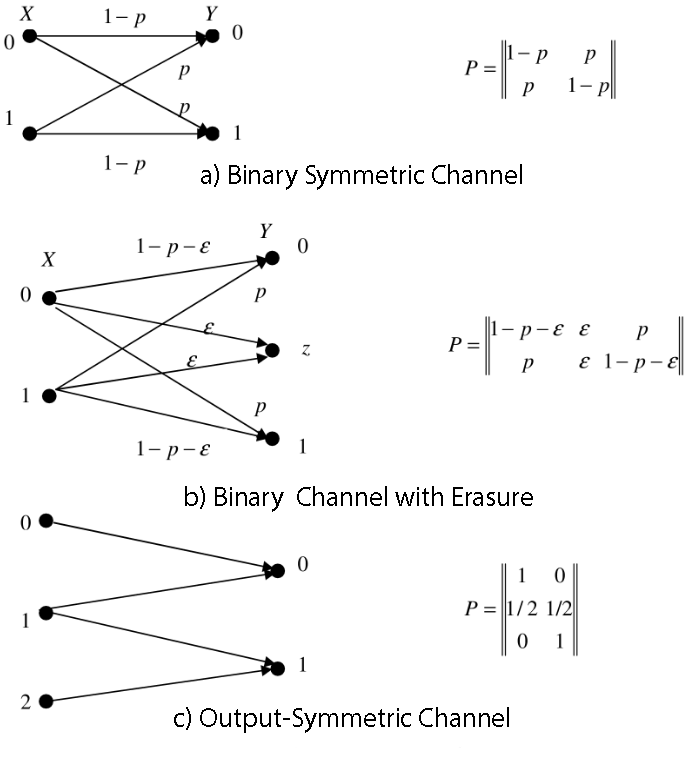
\includegraphics[width=0.65\textwidth]{fig5_8.png}
    %\centerline{\includegraphics[width=3.16in,height=4.02in]
    \caption{Symmetric channels} \label{fig5_8}
    %\end{minipage}
    \end{figure}
\end{itemize}
\end{frame}


\begin{frame}
\frametitle{Symmetrical channels}
Proof of properties
\begin{itemize}
% \footnotesize {
% \small{


    \item[1]
        $I(X,Y) = H(Y) - H(Y\vert X)$. 
        $H(Y\vert X) = \sum\limits_x {p(x)H(Y\vert x)}$
    
    \item[2]
        $H(X) <= \log |X|$
    
    \item[3]
        $p(y) = \sum\limits_x {p(x)p(y\vert x)}$
        $p(y) = \frac{1}{\left| X \right|}\sum\limits_x {p(y\vert x)} , \quad y \in Y $
        $p(y) = 1 / \left| Y \right|$
        
    \item[4] 
        follows from first 1,2,3


\end{itemize}
\end{frame}


\begin{frame}
\frametitle{Symmetrical channels}
\begin{itemize}
% \footnotesize {
% \small{

    \item For a Binary Symmetric Channel: $C_0 = 1 - \eta(p)$
    
    \item Channel is called Generally Symmetric, if bу renumbering it's input characters, it's matrix can be represented as cell matrix
    \begin{equation}
    \label{eq5_41} P = \left[ {\left. {P_1 } \right|\left. {P_2 }
    \right|...\left| {P_M } \right.} \right],
    \end{equation}
    where each sub-matrix $P_i$ is fully symmetric (by input and by output).

\end{itemize}
\end{frame}


\begin{frame}
\frametitle{Symmetrical channels}
\begin{itemize}
% \footnotesize {
% \small{
    \begin{figure}[ht]
    \begin{minipage}{1.0\linewidth}
    \includegraphics[width=0.90\textwidth]{capacity.eps}
    %\centerline{\includegraphics[width=3.16in,height=4.02in]
    \caption{Throughput of Binary Symmetric Channel (BSC)} \label{capacity}
    \end{minipage}
    \end{figure}
\end{itemize}
\end{frame}


\begin{frame}
\frametitle{Symmetrical channels}
\begin{itemize}
% \footnotesize {
% \small{
    \item Binary Channel with Erasure
    \[
    {P}' = \left[ {\left. {{\begin{array}{*{20}c}
    {1 - p - \varepsilon } \hfill & p \hfill \\
    p \hfill & {1 - p - \varepsilon } \hfill \\
    \end{array} }\mbox{ }} \right|\mbox{ }{\begin{array}{*{20}c}
    \varepsilon \hfill \\
    \varepsilon \hfill \\
    \end{array} }\mbox{ }} \right].
    \]
    
    \item Both sub-matrixes are fully symmetric (by input and by output). Thus, Binary Channel with Erasure is Generally Symmetric.

\end{itemize}
\end{frame}


\begin{frame}
\frametitle{Symmetrical channels}
Property 5.
% \footnotesize {
% \small{
    \begin{prop}\label{pr5_5}  
    For Generally Symetric Channel, maximum of mutual information between input and output (see. (\ref{eq5_39})) is achieved when input alphabet characters have equal probability.
    \end{prop}
\end{frame}




\begin{frame}
\frametitle{Symmetrical channels}
Proof of property 5.
\begin{itemize}
% \footnotesize {
\small{
   
    \item Consider transition probability matrix, $Y_1 ,...,Y_M $, $P_1 ,...,P_M $. 
    \item consider entropy of $Y$:
    \begin{equation}
        \label{eq5_42} H(Y) = - \sum\limits_{i = 1}^M {\sum\limits_{y \in Y_i } {p(y)\log p(y)} } .
    \end{equation}
    
    \item Denote 
    \[
    q_i = \sum\limits_{y \in Y_i } {p(y)}
    \]
    
    \item Conditional probability of subset $Y_i $ when $x$ is known:
    \[
    {\rm P}(Y_i \vert x) = \sum\limits_{y \in Y_i } {p(y\vert x)}
    \]  
    
}
\end{itemize}
\end{frame}



\begin{frame}
\frametitle{Symmetrical channels}
\begin{itemize}
% \footnotesize {
\small{    
    
    
    
    \item $\forall x$ holds ${\rm P}(Y_i \vert x) = q_i $.

    \item transform (\ref{eq5_42}):
    \begin{equation}
    \label{eq5_43} H(Y) = - \sum\limits_{i = 1}^M {q_i \sum\limits_{y
    \in Y_i } {\frac{p(y)}{q_i }\log \left( {\frac{p(y)}{q_i }q_i }
    \right) = H(I) + \sum\limits_{i = 1}^M {q_i H(Y_i )} } } ,
    \end{equation}
    
    \item $H(I)$ is entropy of indices $I$:
    \[
    H(I) = - \sum\limits_{i = 1}^M {q_i \log q_i } 
    \]
    
    \item Entropy of subset $Y_i $:
    \[
    H(Y_i ) = - \sum\limits_{y \in Y_i } {\frac{p(y)}{q_i }\log
    \frac{p(y)}{q_i }}
    \]   
}
\end{itemize}
\end{frame}



\begin{frame}
\frametitle{Symmetrical channels}
Example: Binary Channel with Erasure
\begin{itemize}
% \footnotesize {
% \small{
    
    \item $p_x (0) = p_x (1) = 1 / 2$. 
    
    \item  Use formula of total probability
    \[
    p_y (0) = p_y (1) = \frac{1 - \varepsilon }{2},
    \quad
    p_y (z) = \varepsilon .
    \]
    
    \item Substitute ot mutual information formula
    \[
    C_0 = (1 - \varepsilon )\left( {1 - \eta\left( {\frac{p}{1 -
    \varepsilon }} \right)} \right).
    \]
    \item When $p = 0$ we have:
    \[
    C_0 = 1 - \varepsilon
    \]

\end{itemize}
\end{frame}



\begin{frame}
\frametitle{Forward Coding Theorem}
\begin{itemize}
% \footnotesize {
% \small{

\begin{theorem} {Forward Coding Theorem} For Discrete Memoryless Channel with Information Capacity $C_0 $, $\forall \varepsilon $,$\delta > 0$ $\exists n_0 $, such that $\forall n \in \mathbb{N}, n \ge n_0 $, exists code of length $n$ with code rate $R \ge C_0 - \delta $, and it's average error probability $P_e \le \varepsilon $.
\end{theorem}


\end{itemize}
\end{frame}


\begin{frame}
\frametitle{Forward Coding Theorem}
Proof of Forward Coding Theorem. Proof sketch: 
\begin{itemize}
% \footnotesize {
% \small{

    \item[1.]Build Ensemble of random codes with fixed code length and code rate.
    \item[2.] Specify decoding rule.
    \item[3.] Estimate average error probability on ensemble and prove, that error probability is reduced along with increasing of code length.

\end{itemize}
\end{frame}


\begin{frame}
\frametitle{Forward Coding Theorem}
Proof of Forward Coding Theorem. Step 1
\begin{itemize}

    \item Build codes ensemble. Denote as ${\vec p} = \{p(x),x \in X\}$ the probability distribution on $X$, which implies $C_0 = I(X,Y)$:
    \[
    {\vec p} = \arg \mathop {\max }\limits_{\vec p = \{p(x)\}} I(X;Y).
    \]
    
    \item When code rate $R$ and code length $n$ are known, numer of codewords is $M = 2^{nR}$. Choose $M$ such that,
    \begin{equation}
    \label{eq5_44} M - 1 < 2^{n(C_0 - \delta )} \le M.
    \end{equation}

\end{itemize}
\end{frame}


\begin{frame}
\frametitle{Forward Coding Theorem}
Proof of Forward Coding Theorem. Step 2
\begin{itemize}

    \item Decision rule of decoder is stated by splitting $Y^n$ into disjoint $R_m $, $m = 1,...,M$, such that $\bigcup_{m = 1}^{M} R_m = Y^n $, $R_m \bigcap R_{m'} =\emptyset$ при $m' \ne m$. 
    
    \item Use maximum likelihood principle:
    Decision is made in favor of the codeword ${\vec x}_m $, for which $p({\vec y}\vert {\vec x}_m )$ is maximal.

    \item $p({\vec y}\vert {\vec x}_m )$ - likelihood of codeword ${\vec x}_m $. Decision areas of such decoder are:
    \[
    R_m = \left\{ {{\vec y}:p({\vec y}\vert {\vec x}_m ) \ge%
    p({\vec y}\vert {\vec x}_{m'} ),m' \ne m} \right\}.
    \]

\end{itemize}
\end{frame}


\begin{frame}
\frametitle{Forward Coding Theorem}
Proof of Forward Coding Theorem. Step 2
\begin{itemize}

    \item On a $X^n\times Y^n$ define:
    \begin{equation}
        \label{eq5_45} T_n(\theta) = \left\{ ({\vec x},{\vec y}):\left| {\frac{1}{n}I({\vec x};{\vec y}) - I(X;Y) } \right| \le \theta \right\},
    \end{equation}

    where $I({\vec x};{\vec y})$ is mutual information between ${\vec x}$ and ${\vec y}$, and  $\theta \ge 0$ is a cinstant.

    \item  $T_n(\theta)$ is a \emph{set of typical sequence pairs}.

    \item By a received sequence ${\vec y}$, decoder makes a decision in favour ${\vec x}_m $ if $(\vec x_m ,\vec y) \in T_n(\theta)$. 
    
    
\end{itemize}
\end{frame}


\begin{frame}
\frametitle{Forward Coding Theorem}
Proof of Forward Coding Theorem. Step 3
\begin{itemize}    
    
    \item Error is possible in one of this cases:
    \begin{itemize}
    \item
    When sending ${\vec x}_m $, we receive ${\vec y}$, such that $({\vec x}_m ,{\vec y}) \notin T_n(\theta) $.
    \item
    When sending ${\vec x}_m $ we receive ${\vec y}$, such that for some codeword ${\vec x}_{m'}, m' \ne m,$ holds $(\vec x_{m'},\vec y) \in T_n(\theta)$.
    \end{itemize}

\end{itemize}
\end{frame}


\begin{frame}
\frametitle{Forward Coding Theorem}
Proof of Forward Coding Theorem. Step 3
\begin{itemize} 

    \item Denote probability of first case as $P_{em1}$, and probability of the second case as $P_{em2}$. Denote average probabilities as $P_{e1}$, $P_{e2} $. 
    
    \item Estimate error probability:
    \begin{equation}
    \label{eq5_46} P_e \le P_{e1} + P_{e2} .
    \end{equation}

    \item From (\ref{eq5_46}) we get
    \begin{equation}
    \label{eq5_47} \bar {P}_e \le \bar {P}_{e1} + \bar {P}_{e2} .
    \end{equation}

\end{itemize}
\end{frame}


\begin{frame}
\frametitle{Forward Coding Theorem}
Proof of Forward Coding Theorem. Step 3
\begin{itemize}   

    \item 
    \begin{theorem}  \label{typ_pair}
    \small{
        Consider joint probability distribution $\{p(\vec x, \vec y), \vec x \in X^n, \vec y \in Y^n \}$ on  $X^n \times Y^n$, such that:
        
        $p(\vec x)= \prod_{i=1}^{n} p(x_i), \quad
        p(\vec y |\vec x)= \prod_{i=1}^{n} p(\vec y_i | x_i)$. \\
        
        And let $\exists \theta >0$ such that $T_n(\theta)$ is defined by (\ref{eq5_45}). Then holds:
        \begin{enumerate}
            \item $\lim_{n\rightarrow \infty} P\left(T_n(\theta)\right)=1$.
            \item If sequences $\tilde {\vec x}$ и $\tilde {\vec y}$ are chosen from $X^n$ and $Y^n$ respectively with distributions $p(\vec x)$ and $p(\vec y)=\sum_{\vec x} p(\vec x, \vec y)$, then
            \[
            P\left( (\tilde {\vec x}, \tilde {\vec y})\in T_n(\theta) \right)
            \le 2^{-n(I(X;Y)-\theta)}.
            \]
        \end{enumerate}
    }
    \end{theorem}


\end{itemize}
\end{frame}


\begin{frame}
\frametitle{Forward Coding Theorem}
Proof of Forward Coding Theorem. Step 3
\begin{itemize} 

    \item Estimate $\bar P_{e1} $. If $n\ge n_{01}$ holds:
    \begin{equation}\label{pe1}
    \bar P_{e1} \le \frac{\varepsilon}{2} \quad.
    \end{equation}

    \item Estimate $\bar P_{e2}$. Use previous theorem. 
    \begin{equation*}%\label{pe2}
    \bar P_{e2} \le   (M-1) 2^{-n(I(X;Y)-\theta)}.
    \end{equation*}


    \item Having $I(X;Y)=C_0$ and using (\ref{eq5_44}) we get
    \begin{equation*}
    \bar P_{e2} \le 2^{-n(\delta-\theta)}.
    \end{equation*}
    
\end{itemize}
\end{frame}


\begin{frame}
\frametitle{Forward Coding Theorem}
\begin{itemize}
% \footnotesize {
% \small{    
    
    \item Let $\theta=\delta/2$, then $\exists n_{02}$ such that, when $n \ge n_{02}$ holds:
    \begin{equation} \label{pe2}
    \bar P_{e2} \le \frac {\varepsilon}{2}.
    \end{equation}
    
    
    \item (\ref{pe1}) and (\ref{pe2}) imply, that when $n \ge \max \left\{ {n_{01} ,n_{02}} \right\}$, then average error probability is $ \le \varepsilon $. 
    
    \item Thus, at least one of codes in ensemble has error probability $\le \varepsilon $.

\end{itemize}
\end{frame}


% -------------------------Typical Sequence pairs-------------

\begin{frame}
\frametitle{Typical Sequence pairs}
\begin{itemize}
% \footnotesize {
% \small{
    
    \item Denote set of Typical Sequence airs as
    \begin{equation}
        \label{def_typ_p}
        T_n(\varepsilon) = \left\{ ({\vec x},{\vec y}):\left|
        {\frac{1}{n}I({\vec x};{\vec y}) - I} \right| \le
        \varepsilon  \right\},
    \end{equation}
    
    where $I({\vec x};{\vec y})$ -- mutual information between ${\vec x}$ and ${\vec y}$, $\varepsilon$ -- positive constant.

\end{itemize}
\end{frame}


\begin{frame}
\frametitle{Typical Sequence pairs}
\begin{itemize}
% \footnotesize {
% \small{
    Rewrite previous theorem:
    \begin{theorem} {Of Typical Sequence pairs} \label{TYP_PAIR}
    
        $\forall \varepsilon > 0$ holds
        \begin{enumerate}
        \item
        $\lim_{n\rightarrow \infty} P\left(T_n(\varepsilon)\right)=1.$
        \item
        $\tilde P\left(T_n(\varepsilon)\right)\le 2^{-n(I-\varepsilon)}. $
        \item
        $\exists n_\varepsilon$ such that, when $n \ge n_\varepsilon$ holds 
        $\tilde P\left(T_n(\varepsilon)\right)\ge (1-\varepsilon)2^{-n(I+\varepsilon)}. $
        \end{enumerate}
    \end{theorem}
        
\end{itemize}
\end{frame}



\begin{frame}
\frametitle{Typical Sequence pairs}
Proof of theorem of Typical Sequence pairs
\begin{itemize}
% \footnotesize {
% \small{

    \item For arbitrary pairs $({\vec x},{\vec y})$ from  $T_n(\varepsilon)$ holds:
    \[
    I-\varepsilon \le
    \frac{1}{n}\log\frac{p(\vec x,\vec y)}{p(\vec x)p(\vec y)}
    \le I+\varepsilon
    \]
    
    \item or
    \begin{equation}\label{pxpy}
    p(\vec x,\vec y)2^{-n(I+\varepsilon)} \le
    p(\vec x)p(\vec y) \le
    p(\vec x,\vec y)2^{-n(I-\varepsilon)}.
    \end{equation}
    
    \item Probability of $T_n(\varepsilon)$, calculated when ${\vec x}$ and ${\vec y}$ are independently chosen, is
    \begin{equation}\label{pr_typ}
    \tilde P\left(T_n(\varepsilon)\right)= \sum_{( {\vec x}, {\vec y})\in T_n(\varepsilon)} p( {\vec x})p({\vec y}).
    \end{equation}
    
\end{itemize}
\end{frame}



\begin{frame}
\frametitle{Typical Sequence pairs}
Proof of theorem of Typical Sequence pairs
\begin{itemize}
% \footnotesize {
% \small{    
    
    \item Substitute (\ref{pxpy}):
    \begin{eqnarray*}
    \tilde P\left(T_n(\varepsilon)\right)
            &\le&  \sum_{({\vec x}, {\vec y})\in T_n(\varepsilon)}
     p({\vec x},{\vec y})2^{-n(I-\varepsilon)}=
     \\
     &=&2^{-n(I-\varepsilon)} P\left(T_n(\varepsilon)\right)
    \le \\
     &\le&2^{-n(I-\varepsilon)}.
    \end{eqnarray*}

\end{itemize}
\end{frame}



\begin{frame}
\frametitle{Typical Sequence pairs}
Proof of theorem of Typical Sequence pairs
\begin{itemize}
% \footnotesize {
% \small{
    
    \item Analogously,
    \begin{eqnarray*}
    \tilde P\left(T_n(\varepsilon)\right) &\ge&
    \sum_{( {\vec x},  {\vec y})\in T_n(\varepsilon)}
     p({\vec x}, {\vec y})2^{-n(I+\varepsilon)}=
     \\
     &=&2^{-n(I+\varepsilon)}
     P\left(T_n(\varepsilon)\right) .
    \end{eqnarray*}
    
    \item Probability of $T_n(\varepsilon)$ tends to $1$ when increasing $n$, thus $\exists n$ such that it became greater than $1-\varepsilon$. \QED
    
\end{itemize}
\end{frame}


\end{document} 